% This file was created with tikzplotlib v0.9.12.
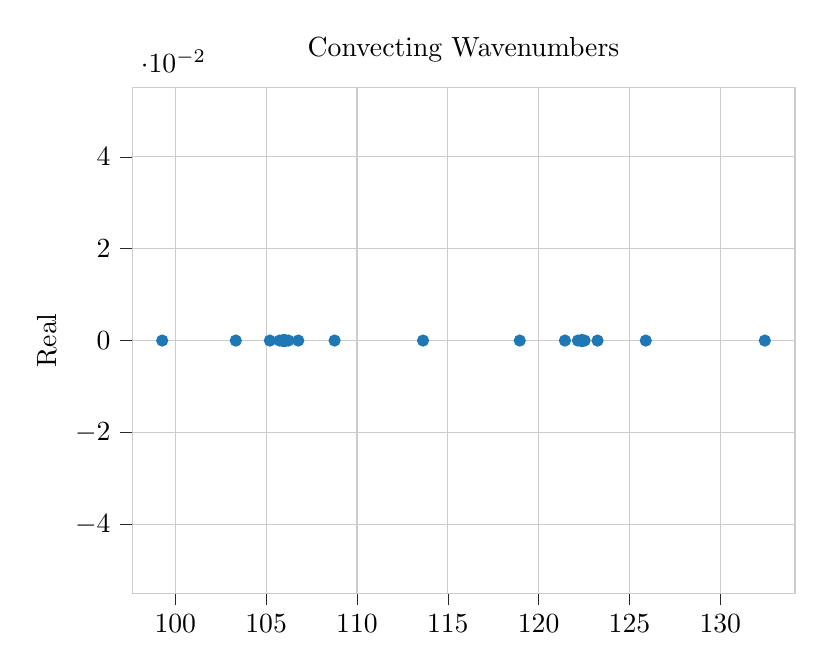
\begin{tikzpicture}

\definecolor{color0}{rgb}{0.12156862745098,0.466666666666667,0.705882352941177}

\begin{axis}[
axis line style={white!80!black},
height=8cm,
tick align=outside,
tick pos=left,
title={Convecting Wavenumbers},
width=10cm,
x grid style={white!80!black},
xmajorgrids,
xmin=97.6197692863098, xmax=134.110291753717,
xtick style={color=white!15!black},
y grid style={white!80!black},
ylabel={Real},
ymajorgrids,
ymin=-0.055, ymax=0.055,
ytick style={color=white!15!black}
]
\addplot [draw=color0, fill=color0, mark=*, only marks]
table{%
x  y
132.451631641562 0
125.897422474376 0
123.243188230366 0
122.530921497709 0
122.368862040143 0
122.33911243426 0
122.339409177868 0
122.345953417978 0
122.353302921341 0
122.360247436777 0
122.366546503833 0
122.37217929712 0
122.377172545049 0
122.381561293117 0
122.385380158661 0
122.388661559083 0
122.391435513702 0
122.39372978231 0
122.395570059455 0
122.396980161992 0
122.397982194725 0
122.398596678456 0
122.398842576431 0
122.398736935489 0
122.398292900754 0
122.397510696659 0
122.396338038959 0
122.394497566757 0
122.390735875143 0
122.379560502826 0
122.337138740825 0
122.161772325606 0
121.44734997074 0
118.961860313411 0
113.637230495131 0
108.768415780809 0
106.769590517171 0
106.222207149804 0
106.088422547892 0
106.054668919973 0
106.044071196157 0
106.038701384846 0
106.034429506614 0
106.030309470328 0
106.026127328692 0
106.021837241715 0
106.017431844947 0
106.012912469632 0
106.008282308208 0
106.003544851731 0
105.998703538146 0
105.993761678238 0
105.988722444768 0
105.983588874959 0
105.97836387246 0
105.97305019492 0
105.967650377357 0
105.962166376962 0
105.956598006949 0
105.950936102155 0
105.945132761291 0
105.938971848429 0
105.931505661672 0
105.91860741024 0
105.882393418363 0
105.746548673262 0
105.205894855093 0
103.328935806445 0
99.2784293984647 0
};
\end{axis}

\end{tikzpicture}
